\documentclass[a4paper,11pt]{article}
\usepackage[top=60pt,bottom=80pt,left=50pt,right=50pt]{geometry}
\usepackage[utf8]{inputenc}
\usepackage[block=space,bibencoding=utf8,style=phys,maxbibnames=6,backend=biber]{biblatex}

\usepackage{multicol}
\usepackage{setspace}
\usepackage{titlesec}
\usepackage{float}
\usepackage{caption}
\usepackage{graphicx}
\usepackage{tcolorbox}

% Math/physics notation stuff
\usepackage{amsmath}
\usepackage{bbold}
\usepackage{amsfonts}
\usepackage{physics}
\usepackage{siunitx}
\usepackage{hyperref}
\usepackage{cleveref}
\usepackage{float}
\usepackage{stackengine}
\usepackage{calc}
\usepackage{xcolor}

% POSTNote formatting and bibfile
\titlespacing*{\section}{0pt}{0pt}{0.3em}
\setlength{\parindent}{0pt}
\setlength{\parskip}{0.5em}
\widowpenalty10000
\clubpenalty10000

% Figures in multicols...
\newenvironment{Figure}
  {\medskip\noindent\minipage{\linewidth}}
  {\endminipage\medskip}

\addbibresource{MPhys.bib}

% Underlining, other notation and convenience commands
\stackMath
\newcommand{\suf}[2]{\stackunder[0.5pt]{\stackunder[1pt]{\ensuremath{#1}}{\rule{\widthof{\ensuremath{#2}}*\real{0.9}}{.1ex}}}{}}
\newcommand{\duf}[2]{\stackunder[0.5pt]{\stackunder[0.8pt]{\stackunder[1pt]{\ensuremath{#1}}{\rule{\widthof{\ensuremath{#2}}*\real{0.9}}{.1ex}}}{\rule{\widthof{\ensuremath{#2}}*\real{0.9}}{.1ex}}}{}}
\newcommand{\su}[1]{\suf{#1}{#1}}
\newcommand{\du}[1]{\duf{#1}{#1}}
\newcommand{\ssu}[1]{\scriptsize\su{#1}\normalsize}
\newcommand{\sdu}[1]{\scriptsize\du{#1}\normalsize}

\newcommand{\nn}{\ensuremath{\su{n}}}
\newcommand{\QQ}{\ensuremath{\du{Q}}}
\newcommand{\dudelta}{\ensuremath{\du{\delta}}}
\newcommand{\ddelta}[4]{\ensuremath{\delta_{#1#3}\delta_{#2#4} + \delta_{#1#4}\delta_{#2#3}}}

\newcommand{\onedot}{$\mathsurround0pt\ldotp$}
\newcommand{\cddot}{\mathbin{
    \vcenter{\baselineskip1ex \vspace{-0.1ex}\hbox{\onedot}\hbox{\onedot}}
}}


\begin{document}
\clearpage
\vspace*{\stretch{2}}
\begin{center}
    \begin{minipage}{.6\textwidth}
        \begin{center}
            \Large
            \emph{Note to editor (marker):}
        \end{center}
        The following couple of pages are intended as a short educational article for a popular science magazine such as \href{https://www.popsci.com/}{Popular science} or \href{https://institutions.newscientist.com/}{New scientist}. Or perhaps even more appropriately for a magazine such as \href{https://chalkdustmagazine.com/}{Chalkdust} which focuses on mathematics and really aims to teach something.
    \end{minipage}
\end{center}
\vspace{\stretch{3}}
\clearpage
\newpage

\begin{center}
    \Huge \textbf{Using Tensors to Model Liquid Crystals}
    \vspace{1em}
\end{center}

\begin{multicols}{2}
    Over the past couple of decades tensor-based approaches to modelling liquid crystals have become dominant.
    In this article we explain how these work and their benefits in order to provide a peak at liquid crystal physics and perhaps demystify the word tensor without resorting to rigorous mathematics and definitions.

    \section*{Liquid crystal phases}
    In the simplest (and dominant) case, liquid crystals are phases of rod-like constituent molecules.
    These molecules are characterized by a single axis of symmetry, perhaps looking like a cylindrical rod, and importantly by both ends looking the same.
    This means that we can rotate any of the molecules by any angle around its axis of symmetry, or flip it by 180\si{\degree} around its middle, and we couldn't tell the difference.
    These operations constitute the symmetries of our system, and they play a big role in determining what any phases may look like.

    While these symmetries may seem arbitrary, they have been observed in many real-world substances.
    Even if the constituent molecules of a substance do not actually look like rods, they may interact with each other in a way that makes them look like these symmetric rods to each other, leading to the discussed symmetries being respected.

    What phases of these substances may look like is best shown visually, see \cref{fig:phases}.
    There two of the phases may be recognizable, the ordered crystalline phase and the chaotic liquid.
    As we allude to, order is the key feature distinguishing the phases.
    In the crystalline phase, we know exactly where every molecule ought to be and in which direction it will be pointing.
    In the language of physics, we have full positional and orientational order.
    In contrast, in the isotropic liquid phase all the molecules are at completely random places and pointing in random directions, we have no order.
    As an aside, the word isotropic means that the system has no orientation to it.

    Finally, our liquid crystalline phases lay between these two extrema, they each feature some level of order which leads to their characteristic features.
    In the nematic phase (\cref{fig:phases}(b)), which is generally the first to form from a liquid at the right conditions,
    \begin{Figure}
        \centering
        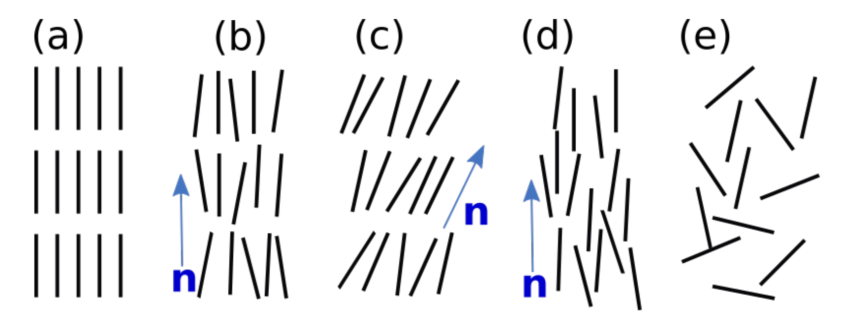
\includegraphics[width=0.95\textwidth]{figures/phases.pdf}
        \captionof{figure}{
            The different phases of a substance of rod-like molecules, in order of increasing order.
        }\label{fig:phases}
    \end{Figure}
    \begin{figure*}[th]
        \centering
        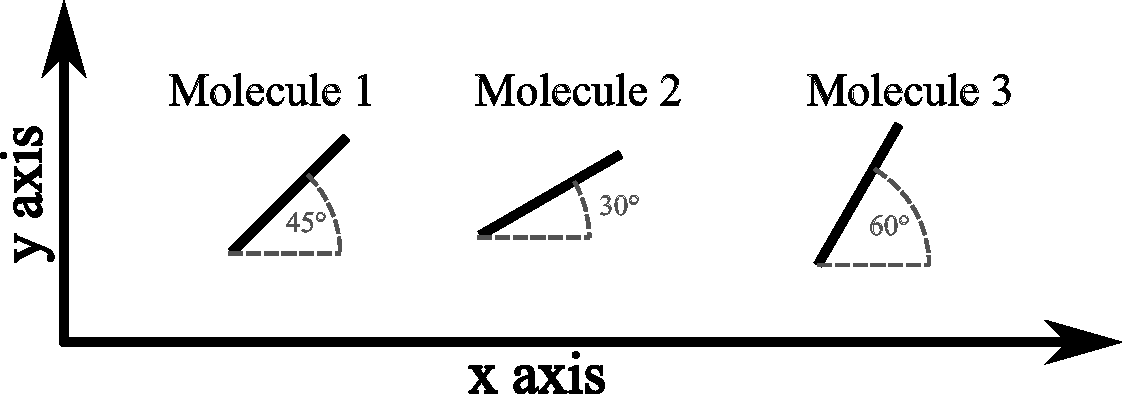
\includegraphics[width=0.85\textwidth]{figures/mols.pdf}
        \caption{
            Example orientations of three rod-like molecules at angles to the x axis.
        }\label{fig:mols}
    \end{figure*}
    the molecules start aligning to each other.
    In a perfect nematic all the molecules of a system would be pointing in exactly the same direction, however they would still be scattered at random positions.
    As such, the nematic phase is defined by orientational order, but no positional order.

    The smectic phase (\cref{fig:phases}(c)) is the next step in order and almost always build on top of the nematic order.
    Its distinctive feature is the formation of layers, so we end up with positional order in the direction of layering.
    However, true smectics do not have any order within the layers, they may be viewed as defined stacks of two-dimensional disordered liquids.

    % There are other more ordered liquid crystalline phases along with there being a myriad of subtypes of nematic and in particular smectic phases.
    % Howeverm
    
    \section*{Modelling nematics}
    We want to describe whether molecules of a system are aligned and perhaps also in which direction they point.
    % In a real-world system our substance of rod-like molecules could well have sections of it that exhibit nematic order in one direction and another section which is aligned in a different direction.
    Now in a real-world scenario our system way very well form multiple domains that exhibit nematic order in different directions with boundaries between them.
    However, let us first consider a small system which if nematic will only fit one such domain.

    \subsection*{Using vectors}
    Ultimately, we first need to quantify the orientations of each of our molecules.
    In physics the most common approach to such problems is to use vectors.
    One of the most intuitive ways of thinking about vectors is that they represent both a magnitude and a direction.
    They can then be represented themselves either by arrows in diagrams or perhaps as sequences of numbers.
    In our case we use unit vectors, vectors with magnitude 1, which only carry a direction.

    To see how this cann be done, consider the three example molecules in \cref{fig:mols}.
    We may represent the directions of each of the molecules as
    \begin{align*}
        \su{n}_1 \leftrightarrow \frac{1}{2} \begin{pmatrix} \sqrt{2} \\ \sqrt{2} \end{pmatrix} && 
        \su{n}_2 \leftrightarrow \frac{1}{2} \begin{pmatrix} \sqrt{3} \\ 1 \end{pmatrix} &&
        \su{n}_3 \leftrightarrow \frac{1}{2} \begin{pmatrix} 1 \\ \sqrt{3} \end{pmatrix}
    \end{align*}
    with the top component of each pair of numbers corresponding to how much of the molecules length points in the x direction and the bottom component is analogous but for the y direction.
    You don't have to understand why its specifically these numbers, but hopefully you can see how they seem to correspond to the directions of \cref{fig:mols}.
    In addition, they all have the property that the x component squared plus the y component squared is one, this corresponds to the mentioned magnitude of 1.

    \raggedcolumns
    Similarly, we can always associate a vector \nn\ to any such a molecule, and then we can look at if these vectors of nearby molecules look similar and so they are aligned.
    However, there is a problem with this approach, see vector components are allowed to be negative (they have to, otherwise we could not describe a molecule perpendicular to molecule 1).
    Given that, molecule 1 could equally well be described by
    \begin{equation}\label{eq:dyad}
        \su{n}_1' = -\su{n} \leftrightarrow \frac{1}{2}\begin{pmatrix} -\sqrt{2} \\ -\sqrt{2} \end{pmatrix}
    \end{equation}
    which in numerical terms is very far from the original \nn.
    This problem really corresponds to the mentioned symmetry of the cylindrical molecules, an essential feature of many liquid crystals.

    \subsection*{Using tensors}
    This is where tensors come in.
    In this case they really may be thought of as matrices where we the core ingredient is the matrix given by
    \begin{equation*}
        \du{M} \leftrightarrow \begin{pmatrix}
            n_1\times n_1 & n_1\times n_2 \\ n_2\times n_1 & n_2\times n_2
        \end{pmatrix}
    \end{equation*}
    with $n_1$ and $n_2$ being the top and bottom components of \nn.
    This matrix has the crucial benefit of being the same if we switch \nn\ to -\nn\ as before.
    In practice a slightly different matrix is used given by
    \begin{equation}\label{eq:kaka}
        \du{Q} = \du{M} - \frac{1}{2}\begin{pmatrix} 1 & 0 \\ 0 & 1 \end{pmatrix}
    \end{equation}
    which still has the same important property.

    For the three molecules of \cref{fig:mols} we then have
    \small
    \begin{align*}
        \QQ_1 \leftrightarrow \frac{1}{2}\begin{pmatrix} 0 & 1 \\ 1 & 0 \end{pmatrix} &&
        \QQ_2 \leftrightarrow \frac{1}{4}\begin{pmatrix} -1 & \sqrt{3} \\ \sqrt{3} & 1 \end{pmatrix} &&
        \QQ_3 \leftrightarrow \frac{1}{4}\begin{pmatrix} 1 & \sqrt{3} \\ \sqrt{3} & -1 \end{pmatrix}
    \end{align*}
    \normalsize
    and in order to gauge how aligned our molecules are and so how nematic our system is, we take the average of all the molecule \QQ\ tensors
    \begin{equation*}
        \QQ_\text{avg} = \frac{1}{3} (\QQ_1 + \QQ_2 + \QQ_3) \leftrightarrow \frac{1 + \sqrt{3}}{6} \begin{pmatrix} 0 & 1 \\ 1 & 0 \end{pmatrix}
    \end{equation*}
    and then put it in a form resembling \cref{eq:kaka} for interpreting, in our case this is
    \begin{equation*}
        \QQ_\text{avg} \leftrightarrow \frac{1+\sqrt{3}}{3}\qty(\frac{1}{2} \begin{pmatrix} 1 & 1 \\ 1 & 1 \end{pmatrix} - \frac{1}{2}\begin{pmatrix} 1 & 0 \\ 0 & 1 \end{pmatrix})
    \end{equation*}
    where the number $\frac{1+\sqrt{3}}{3}$ is called the nematic order parameter $S$ and the first matrix corresponds to the overall phase orientation.
    Specifically, we deconstruct the matrix into a vectorial direction in the same way we originally formed a tensor from a vector, via \cref{eq:dyad}.
    In this case it is easy to verify that it corresponds to a vector
    \begin{equation*}
        \nn \leftrightarrow \pm \frac{1}{2}\begin{pmatrix} \sqrt{2} \\ \sqrt{2}        \end{pmatrix}
    \end{equation*}
    and hence the same orientation as molecule 1.
    Which intuitively makes sense as the other two molecules are each rotated by 15\si{\degree} in either direction, so their effect cancels out.

    However, where there effect does not cancel out is the nematic order parameter $S$.
    Due to how the math of the averaging works out this is always restricted to be between 0 and 1.
    We get $S=1$ for a full nematic phase where all molecules point in exactly the same direction, and $S=0$ for an isotropic liquid with random orientations.
    In our case we have $S\sim0.91$ which corresponds to a very well aligned, but not perfect nematic.

    \section*{Conclusion}
    As we have illustrated, using a tensor quantity to represent the orientations (as opposed to vectors) of rod-like molecules comes with the major benefit of faithfully representing their symmetry.
    The nematic \QQ\ tensor and convenient math briefly introduced by example has been well established since the last century and is nowadays the standard method for describing nematics.

    In addition, lately a new approach to modelling smectic layering using a tensor called $\du{E}$ has been developed.
    There again the tensor better respects the symmetry of an orientation-like quantity, the layer normal direction.
    In essence the symmetry of smectics boils down to layering upwards and downwards being the same thing, as such we have the same exact symmetry as before and using a tensor instead of a vector is a natural next step.


\end{multicols}


% \newpage

% \textbf{I know there's some bad formatting in the references, I'll fix that}

\end{document}
